% Main Document for PyBP
\documentclass{ctexbook}
\usepackage{amsmath}
\usepackage{float}
\usepackage{subfigure}
\usepackage[pdftex,
            bookmarksnumbered,
            bookmarksopen,
            CJKbookmarks,
            colorlinks,
            citecolor=blue,
            linkcolor=blue,
            ]{hyperref}
\usepackage{tikz}
\usetikzlibrary{positioning,shapes,shadows,arrows}

\usepackage{booktabs}
\usepackage{multirow}
\usepackage{slashbox}
%\usepackage{listings}
%\usepackage{authblk}
\usepackage{color}
\usepackage{lscape}
%\usepackage{syntonly}
%\syntaxonly

\title{Python for Brain Parcellation}
\author{Neuroimaging and Informatics Team}
\date{\today}
\begin{document}
\maketitle
\frontmatter


\tableofcontents
\listoftables
\listoffigures
\mainmatter

\chapter{PyBP ʹ��}
\section{PyBP �����ֲ�}
\subsection{PyBP����}
Ϊʹ��PyBP����������~/.bashrc�н����������ã�
\begin{enumerate}
\item ����Python·��������Python�����ҵ�PyBP��\\
    PYBP=\~/workingdir/svn/neospearman/toolbox/pybp/tags/pybp\_latest
    PYTHONPATH=\$PYBP:\$PYTHONPATH
    export PYTHONPATH

\item ����ϵͳ·��������ϵͳ�����ҵ�pybp��pybp-sess��\\
    PYBPBIN=\~/workingdir/svn/neospearman/toolbox/pybp/tags/pybp\_latest/bin
    PATH=\$PYBPBIN:\$PATH
\end{enumerate}

\subsection{�淶}
\begin{enumerate}
    \item ��������ͳһ�趨ΪZ=2.3��
    \item ��ɵ�ROI��ͳһ����Ϊ \textbf{��������������ĸСд}��\_labelname\_thr.nii.gz����ʽ,��zzl\_face\_z2.3.nii.gz��
\end{enumerate}

\subsection{����}
\begin{enumerate}
    \item ����sesspar(session parent directory)��sessid(session identifier)�ļ���sesspar��sessid�ļ�������Ϊ���⣬ֻҪ�ļ��б������session parent directory��session identifier ���ɣ�
    \item ͨ�������������������pybp-sess -df atlaspar -sf G1 -c face-object -stat zstat1.nii.gz -lt 2.3 -ht 5 -labelvol face.nii.gz -label face -o zzl\_face\_z2.3��
    \item ʹ��watershed ��zstat1���зָ�õ�zstat1\_ws��
    \item ������ʾ˳��MNI�������²㣬�ϱ�����Ϊzstat1,zzl\_face\_z2.3,face,��zstat1\_ws�������ֻ��ʾ�ض�Label, �ɵ���face.nii.gz��colormapΪsingle ROIģʽ��
    \item ѡ��zstat1\_ws,Ϊ��ǰ����ͼ�񣬲�ֵ�����ϲ㣻
    \item ��Label Config Centerѡ��ǰҪ����ROI��
    \item ��������������ROI toolset��������Target volume Ϊ zzl\_face\_z2.3��
    \item �ڵ�ǰ����ͼ���ϣ�ѡ���Ŀ��ROI��Ӧ��cluster�����������ѡ����ʹ��Deselectѡ�����ѡ����ɺ���run,��ɸ�ROIѡ��
    \item ͬʱ��ʾzstat1��face.nii.gz��zzl\_face\_z2.3�����ջ�ROI�Ƿ���ȷ��Ҳ��ѡ��������ROI����ɺ�ͳһ��飻
    \item �ص���6������ʼ����һ��ROI��
    \item �������ROI��ͬʱ��ʾzstat1��face.nii.gz��zzl\_face\_z2.3���������ѻ�ROI�Ƿ������������Lightbox View�� Orth View������·ֱ����£�ȷ������ROIλ��û�����⡣
\end{enumerate}

\subsection{����}
\begin{enumerate}
    \item PyBP��������������������ȷ��label config center �������label����ʾ������
    \item ����ʱ�����ҶԳ�ROI��һ��Ҫͬʱ���й۲��ѡ��ǧ���ȫ���������Ժ���ȥ�����ԣ�
    \item �ж�һ��watershed cluster�Ƿ�������Ҫ����ROI������Ҫ�۲����Label�����ж��ͬʱҪ�۲��cluster�����ڶ���ϵ�����
    \item STS ���cluster��ʱ��Ϊ��ɢ��ѡ��ʱע�����򣬶Գ��Ե�����������
    \item ��������󲿷��ڰ����е�cluster����Ҫѡ�������һ��cluster�Ȱ���λ�ú��ʵĻ��ʲ��֣�Ҳ�а��ʲ��֣���Ҫ����ѡ��
    \item ��һ��ROI(label)�У����ڶ��clusterʱ����λ�ú��ʣ���cluster������������ѡ��
        ���cluster�໥���룬��cluster��С��࣬Ҳ����ѡ��������룬�Ҵ�С���ܴ󣬿�ֻѡ��ϴ�ġ�
    \item ����Ĭ��watershed sigma=1ʱ���ֱ�Ӧ��Ϊ���cluster�Ĵ�cluster����ֱ��ѡ�������cluster����������ʱ����ͨ���ֶ�����sigma=0��������Ƿ����⣬������⣬��ROI��
���Ի���sigma=0����ѡ�����sigma=0�Բ����⣬����Ҫ�ֶ�������������
    \item ʹ��Label single ROI��ʾģʽ����ʹ���ǹ�עij���ض�ROI������Ҳ��ζ��ʧȥ�˺�����label�����λ�òο���Ϣ�����޷��ж�ij��cluster�����ڵ�ǰROI����������ROI��
        ���԰�face.nii.gz��face����ʾģʽȫ����ʾ�����������жϣ�
    \item ���о�watershed clusterȫ����ʾ�Ƚϻ��ң�����ͨ��ROI filter���ܰѺ�Ŀ��ROI�ཻ������cluster��filter��һ����volume�У�Ȼ�����ѡ��
    \item ʹ��pybp-sessʱ������ͨ��sessid�ļ�������ÿ��Ҫ����Щ���Ե�ROI������segid������԰����sessid�ļ����飻
    \item ��ʼѡ��һ��ROIʱ������ȷ��Label config center���Ѿ��Ƶ���ROI��
    \item ʹ��ROI toolset�ڶ�cluster����labeling��ʱ������ȷ��target volume��ȷ��Ȼ���ٽ���clusterѡ��
    \item ���ʱ��һ��Ҫ��ѡ�õ�ROI���ͼ���ͼ�໥�Ƚϣ�
    \item ��ϸ����ʱһ��Ҫ�۲���ϸ���ۺϿ��Ƕ෽����Ϣ����λROI��
    \item ����Ҫ��ȥ���������Լ����жϣ����ܾ����Լ��Ƿ�ѡ����ȷ��ֻҪ�����ͺá�
\end{enumerate}


\section{ROI��Ϣ}
\subsection{�����ο�}
    \begin{enumerate}
        \item ��׼�ṹ��MNI152�����ṩ��۽���λ�úͷ�Χ��Ϣ;
        \item ����ʷ�����group level parcellation�����ṩ����λ�úͷ�Χ�ο���
        \item �����ͼ��probabilistic map���� �ṩ�˼������ǿ����Ϣ, �����ݾ������ֵ�������ò��󣬶��������Եļ���ֵ���ø���
        \item ���弤��ͼ��subject-specific activation map���� �ṩ�������Լ���ǿ����Ϣ��
    \end{enumerate}

\subsection{����ȷ��׼��}
\begin{enumerate}
           \item ������ͼ�����ڽ���������landmark������λROI��
           \item ����ָ�������group parcel����������λROI;
           \item �ڳ���ȷ��ROI cluster�󣬲�ͬROI������λ����Ϣȷ��ROIѡ����ȷ��
           \begin{enumerate}
               \item ������ӦROI�����Գƣ�
               \item Faceϵͳ�У�OFAһ��λ��pFus�ĺ�б�Ϸ���pFusλ��aFus�ĺ�б�Ϸ�����STS�����λ��pFus��aFus�Ϸ�ƫ���ĵط���
               \item Objectϵͳ�У�LOλ��pFs���Ϸ�ƫ����λ�ã�
               \item Placeϵͳ�У�TOSλ��Ƥ���⣬��Լ��RSC�Ϸ��Ժ�ƫ��ࣻRSC��PPA��ȣ��Կ��ڲ�ƫ�ϡ�
           \end{enumerate}
\end{enumerate}



%\chapter{Development}
\section{BP Design or Refactor}
\begin{enumerate}
 \item Ŀ��
\begin{enumerate}
    \item �õĿ�ܣ��׶�����д������չ����ά�������ã�
    \item �õı�׼����Чʵʩ�Ļ���
    \item �õĹ��ܣ����á��๦�ܣ�
\end{enumerate}

 \item �ֶ�
\begin{enumerate}
    \item �����ع�(OOP + DP)
    \item ��ȷ���󣬻ص�����Ӧ��
\end{enumerate}

 \item ��׼(��������)
\begin{enumerate}
    \item Design�����嵽�ӿڲ�������Щ�޷�������࣬�������о����ʵʩ��
    \item Coding: ����淶������������������������׼��
    \item Testing: ���Թ淶��������׼��
    \item document: �ĵ��淶��������׼��
    \item collaborating: Э����ʽ����ɫ(�����ߡ������ߡ�ʵʩ��):�ֹ�Ӧ��ȷ�����帺����Щ�࣬������ķ�����
\end{enumerate}


\item BP ����
���ڸ����ĵ�ģ����ģ���ݣ�����ͼ�ף��ܸ��Ӻ����Ķ�λ�������ԵĹ�����
\begin{enumerate}
    \item ���ڵ�ģ�Ͷ�ģ�����ֶ��ָ������������״������������ԣ���
    \item ���ڵ�ģ�Ͷ�ģ���������Զ��ָ����������
    \item �������л�ָ�õ���Label ����ROI����(�ź���ȡ,mean,std)��
    \item �������л�ָ�õ���Lable �������ӷ���(�ź���ȡ,mean,std)��
\end{enumerate}

\item Issues to resolved
\begin{enumerate}
    \item samples vs features:
    \begin{enumerate}
        \item ��Ϊfeature,ÿһ����һ����������Ϊsample��ÿһ����һ��voxel.
        \item chunk: voxel vs. TR, region vs. run ,  whole volume vs session .
    \end{enumerate}
    \item Pipeline:
    \begin{enumerate}
        \item Unsupervised segmentation: segrep = segmentationReproducibility(segmentationMachine, partitioner(), reproducibilityMetric)
        \item Supervised segmentation:   segpred = segmentationPerformance(segmentationMachine, partitioner(), predictionMetric)
        \item segmentationReproducibility �� cross-validation������ reproducibilityMetric �� error ������partitioner ��
        \item image segmentation vs. machine learning(clustering \& classification) vs. energy optimization��train, predict�������ߵĺ���
    \end{enumerate}
    \item Multimodality info:
    \begin{enumerate}
        \item ʹ��ͳ�Ʒ�������ʽ��ȡ��Ϣ-clustering and classification
        \item �������캯������ʽ��ȡ��Ϣ-energy function
    \end{enumerate}

     \item ID based(freesurfer annotation) vs. location based(fslview); morphology vs. statistic vs. label

     \item functional region vs. functional landmark
\end{enumerate}


\item GUI Issues
\begin{enumerate}
    \item New ROI Unit
    \item ROI operator
    \item Automatic ROI
\end{enumerate}

\vspace{5\baselineskip}

\item LTM study
\begin{enumerate}
    \item ʹ��maximization of consistency �Ż�ROI�����壺consistency һ�´�����������ô�����Ǹ����ĵ������Dz�ͬvoxel�����Բ�һ�£��������ڲ�ͬ������voxel��
    \item ��Ҫtask fMRI �������ʱ����Ҫ�Ż�ô��������ֵ������Ϊͼ���������ģ��Ǿ�Ӧ��ֱ����peak�㣬������ȡ�������㡣��Ϊ��ʱ���ֵ��ĸ��ֲ�һ�£�����������variability�������ϣ����ֲ�����Ӧ���Ǹ�����ģ�ͣ�group template��Ӧģ�;�ֵ��Ȼ��ÿ�������Ǵӷֲ��г��������variability
    \item ��ͬ�������õ���Ҫ��ɶ�� ȱ��controlģ�ͣ���������������ʼ����ЧӦ+�ռ�Լ�������á�
    \item ��λ��ڶ���������������ֲ�ͬvoxel��ģ�ͣ�
\end{enumerate}

\item KXZ \& WX
\begin{enumerate}
    \item ���ڶ�ģ̬������ȷ����ͬ�Թ������߽磬������Լ������ν��������ָ
    \item ���ڶ�ģ̬���������ڱ�������С����ʹ�ö���ģ̬��Ϣ�Ż�peak�㣬������Լ�����ҵ������أ�
    \item ���ڶ�ģ̬�������ϲ���ͬcontrast�õ���peak�㣬�����о���࿿����Զ���ϲ�peak�㣬��û����������Ϣ��
    \item ���ڶ�ģ̬����������Group ROI�Ż���������ROI,��ȷȷ��ROI��������Լ������ν�����׼��
    \item ���ڶ�ģ̬����������fMRI��ͬ����overlap����(��FFA and EBA)������ⲿ����ƽ������Ѫ����ɢ���£��Ƿ��ڸ��ߵ�MRI��DTI�ֱ����£�������߶�λ�ľ��ȣ�֤��������overlap��
    \item ���ڶ�ģ̬����������Ԥ��ģ��Ԥ���±�������(�ռ�Ŀ��)�����������ǣ�����ʲô��������ͼ�׼���ι��죺
    \begin{equation*}
        p(ffa|conn)  = \frac{p(conn|ffa)*p(ffa)}{\int{p(conn|ffa)*p(ffa)}}
    \end{equation*}
\end{enumerate}


\item ���㷶��˼��
\begin{enumerate}
    \item ��֪������Ϣ����ΰ�����������ȡ�����飿
    \item ��֪�ṹ���ӣ���ΰ�����⹦�����ӣ�
    \item ��֪��������֪���ӣ�
    \item ����ں����Ӻͼ���ʹ�����Ӽ�����ͬ���ԣ�������ǿ�ȣ�
\end{enumerate}



\item �ֹ�
\begin{enumerate}
    \item ������,������,Ѧ��ɽ-framework, image segmentation;
    \item ������,������-manual segmentation;
    \item ������-Multimodality(DTI,rfMRI) based brain parcellation;
    \item ����-Multimodality(DTI,rfMRI) based brain parcellation;
    \item ������-Database and text analysis
\end{enumerate}


\item Package
\begin{enumerate}
    \item datasets(IO)
    \item measures(neighbor, set or image (dis)similarity)
    \item Algorithms(segmentation, clustering and classification)
    \item parcel(cluster, peak and manual roi making, roi temporal and spatial statistic like anatomy toolbox)
    \item stats( statistic for ROIs)
    \item editor \& viewer(display image and signal)
\end{enumerate}

 \item Data model for processing
\begin{enumerate}
\item Raw data: MRI(thick,...),Task fMRI(activation,conn),Rest fMRI(conn), DTI(fa,conn)...;
\item Parcel: ROI, cluster, atlas
\item Data format: NII, other format(txt, npz) for  intermediate data(connectivity, roi feature) and attributes
\item Attributes for input data
        \begin{enumerate}
            \item image info: volumedim, voxelsize, voxel
            inchies,mask, space(native vs. MNI),rep(volume vs. surface)
            \item conditional attributes: ca
            \item feature attributes: fa(thickness, FA, activation)
            \item sample attributes: sa(chunk for group, identifier for clustering)
            \item data attributes: da(imghdr,mapper)
        \end{enumerate}

\item Attributes for output parcel:
            \begin{enumerate}
                \item label name, number of label,
                \item label type(statistic vs. label,macro vs.micro, function vs. anatomy)
                \item deriveddata,derivedmethod, derivedpara
                \item temporal and spatial statistical information(size,volume,max,min)
            \end{enumerate}
\end{enumerate}

 \item measures
\begin{enumerate}
    \item neighbor in volume and surface
    \item set/image/surface similarity(dice...)
\end{enumerate}

 \item Algorithms
\begin{enumerate}
        \item Classifications(supervised classification)(Bayesian, Dictionary learning,Hierarchy model)
        \item clustering(Ncut,GMM,Kmeans and spatial constrain version)
        \item Image processing(image segmentation-watershed,region growing)
        \item Elements of the Algorithms
        \begin{enumerate}
                    \item Measure: similarity or distance measure
                    \item Optimization(Convex Optimization,ML,MCMC)
                    \item Prior: sparse,Neighborhood(pymvpa/mis/neighborhood.py)
        \end{enumerate}
        \item Useful Information
        \begin{enumerate}
            \item image intensities;
            \item global position within the brain;
            \item position relative to neighboring brain structures;
            \item anatomical landmarks.
        \end{enumerate}
\end{enumerate}

 \item Editor
\begin{enumerate}
    \item editor
    \item viewer(display image and signal)
    \item data model for visualization;
    \begin{enumerate}
        \item image type(volume vs. surface, statistic vs. label, native vs. MNI),visibility
    \end{enumerate}
\end{enumerate}
\end{enumerate}


\section{pymvpa}
\begin{enumerate}
    \item base.dataset: attrdataset(class), datasetmethod
    \item dataset.base: Dataset(container): dataset $\rightarrow$ imgdata and patata
    \item mri.fmridataset, eventrelated.erdataset, eep.eepdataset; \_data2img,\_img2data�������ݶ�д, dataset ֻ���� voxel indices
    \item dataset�� mapper(chinamapper,interface), node(chainnode,processing object)��classifer, measure, generator
\end{enumerate}


\section{pybp}
\begin{enumerate}
\item �������
\begin{enumerate}
    \item ���1�� imgdata(imgparcel),surfdata(surfaceparcel), patdata(patparcel)(���ݰ����ռ䣬ʱ�䣬�����ȶ�����Ϣʹ��mapper����������) + dataload(imgload, txtload,surfload)�����������data + datasave(imgsvae, surfsave, txtsave)
    ----pymvpa ֻ��һ��dataset�����������ַ�ʽ������ʺ�����ô��
    \item ���2�� dataset(load,save �ӿ�) $->$ imgdata,surfdata,patdata--ͬ����������mapper���������ݶ�����mapper�ӿ�����ͳһô��
\end{enumerate}

\item patdata��input�ļ���ʽ��ƣ�ǰ����Ϊsample ����x,y,z��Ȼ���ṩpat�IJο�volume or surface����ȡ����������Ϣ���Ӷ����⸴�ӵ��ļ���ʽ��
    \begin{verbatim}
        #the data must be provided with a ref volume
        Datadesp: connectivity/activation/dti
        Session: session name
        Numfeature: ddd
        Numsample: ddd
        Samplespace: volume or surface
        voldims: x y z
        voxsize  x y z
        Coordstype: ijk or ras
        Matrix
        1 2 3 0.1 0.3 0.4
        4 3 2 0.3 0.4 0.6
    \end{verbatim}
\end{enumerate}


\begin{figure}
    \caption{searchlight} \label{fig:01}
    \begin{center}
        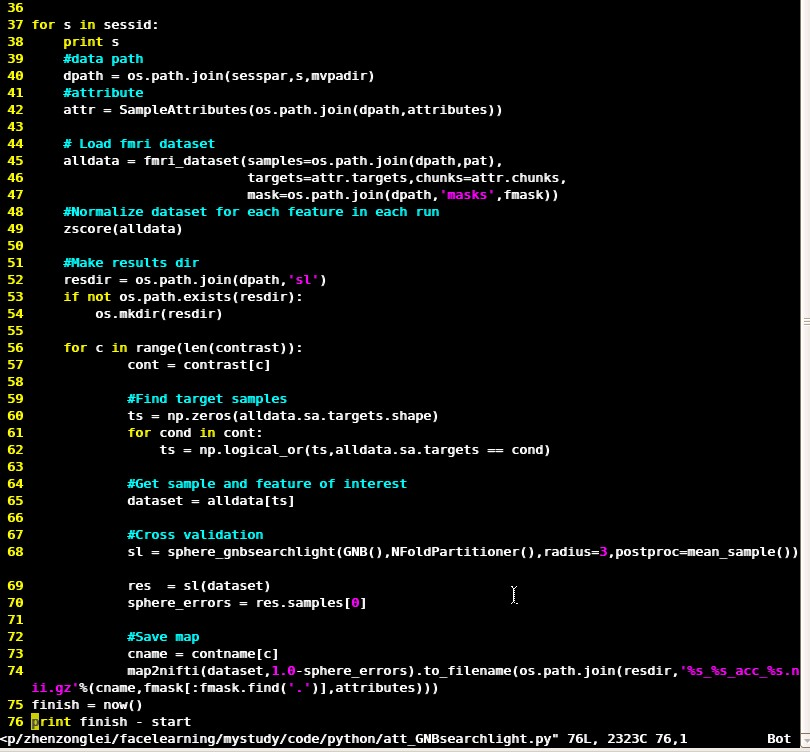
\includegraphics[width= \textwidth]{figure/pymvpasearchlite.jpg}
    \end{center}
\end{figure}

\begin{figure}
    \caption{CV} \label{fig:02}
    \begin{center}
        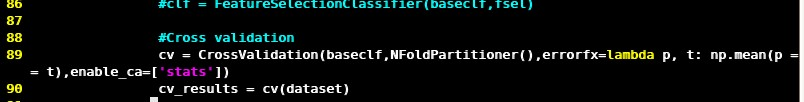
\includegraphics[width= \textwidth]{figure/pymvparoi.jpg}
    \end{center}
\end{figure}


\begin{figure}
    \caption{CV} \label{fig:03}
    \begin{center}
        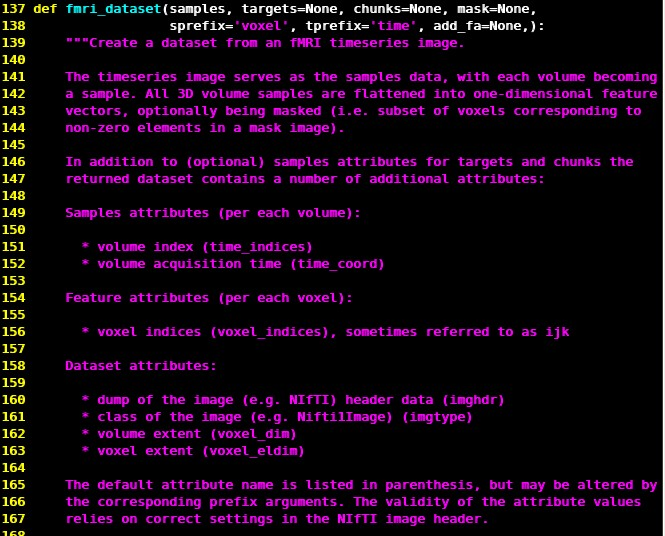
\includegraphics[width= \textwidth]{figure/datasetattr.jpg}
    \end{center}
\end{figure}

\begin{figure}
    \caption{CV} \label{fig:06}
    \begin{center}
        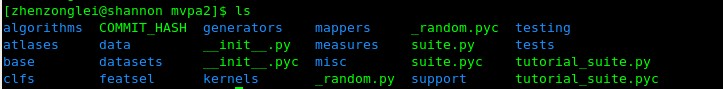
\includegraphics[width= \textwidth]{figure/pymvpapackage.jpg}
    \end{center}
\end{figure}


\begin{figure}
    \caption{CV} \label{fig:04}
    \begin{center}
        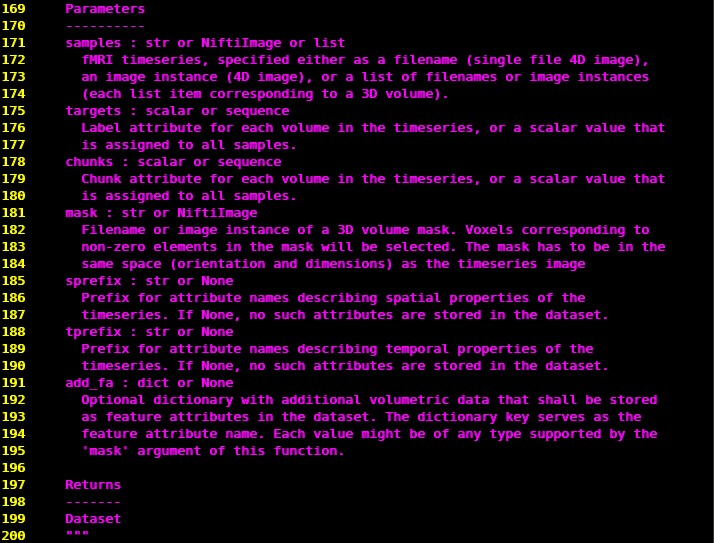
\includegraphics[width= \textwidth]{figure/datasetpara.jpg}
    \end{center}
\end{figure}


\begin{figure}
    \caption{CV} \label{fig:05}
    \begin{center}
        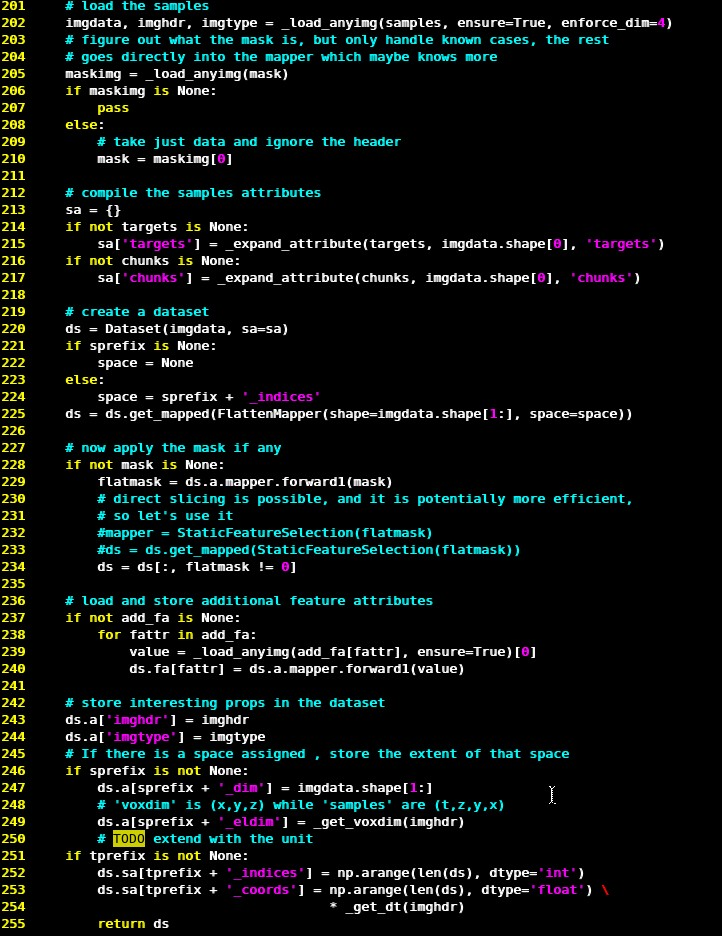
\includegraphics[width= \textwidth]{figure/fmridatasetcode.jpg}
    \end{center}
\end{figure}

\newpage
\section{Development for PyBP}
\subsection{������}
\begin{enumerate}
     \item File: open, save, save as
     \item Volume Edit: create, remove, clone, union, intersect,not, xor, mask,
     \item Preprocessing tool:smooth, sharp, filter, dilate, erosion,opening, closing
     \item Automatic Segmentation: watershed,cluster,region grow,ncut
     \item Manual Segmentation:���voxel �����������brush, pen, rubber
     \item ROI Edit: ���ID�����������merge, split, delete, add(point,box or sphere), label, collect
     \item Color Scheme Edit:
     \item ROI Statistics:
     \item ICA �������飺1)��cluster����overlap����atlas, 2)����ICA ROI ���� VBM
\end{enumerate}


\newpage
\subsection{ZZL}
\begin{enumerate}
    \item �ļ�������File->Open �Ļ��� File->Load volume(surface),save volume
    \item Volume������New image ���� New volume;
    \item ROI������New ROI, Load ROI, Save ROI, Close ROI
    \item Label edit, Voxel edit and ROI edit������ʱ��ѡ���ʲô���в�����Ȼ���г��Ը�����ܵIJ�����voxel edit ��voxelΪ��λ����ROI edit ��ROIΪ��λ������add,delete ROI,name ROI
    \item �޷����������ƿ��ͼ����ʾ��Ĵ�С���Ŵ�����GUIʱ�������ֻ�ǿհ״���

    \item group label����ɫ�ͻ�����ɫһ�£����ѹ۲������Щ���»���ȥ�ģ���Щ��group label������different color scheme or show label outline only �ɽ��
    \item ��ɫ��label�ͼ���ͼ����ɫ��ͻ���޷�������Щ�Ǽ����Щ��label��
    \item ɾ��label ����Ӧ��label �Ͳ�����ʾ�ˣ����ڵײ�ûͬʱɾ��������ճɲ�һ�¡�
    \begin{enumerate}
        \item ���ݺͶ�Ӧ����һ��ɾ��;
        \item ����ʹ�ã�����warning,˵�����label�Ѿ���ʹ�ã��޷�ɾ����
        \item �����Ƿ�ʹ�ã���������ʾ��˵���ܻ�����һ�µ����⣬�û�����֤��label color,ID,name ������Ϊlabel color scheme ���ڣ��Ӷ���ͬ��ID���Բ�ͬ�����ƺ���ɫ��
    \end{enumerate}
    \item �༭�Ƕ�ij����еģ����һ����ı༭�����ܱ༭��һ�㣬����ͬ���ı༭��Ӧ���и�����ȷ�ı߽�;
    \item ���´򿪱�ʱ���ϴε�����size���Ĭ��ֵ1�����м��书�ܻ����Щ��

    \item �ڵ����ϻ�����2D ROI����α�֤��������һ����������: dilate and erode��
    \item add volumeʱ����ȡ�����Ծɱ� can not load warning,�������û�ϰ�ߡ�
    \item ��ά��ʾ����ͼ��ʽ��������Ҫ�ģ�ֻ��axis��ʾ������ȱʧ��λ�У�����posterior sts��anterior sts
    \item ���ѡ��һ��label��ֻ��ʾ�Ǹ�label�������Ǹ�Label�������ڹ�ϵ��cluster���᲻����Ч����ߣ�
    \item ˢ�ӻ�ͼ�꣬����ˢ��״̬�����״̬��Ӧ���в�ͬ����ʾ
    \item ����Ǹ��б��հ�̫�����ɿ����Ż��ռ䣻������һ�е���ʽ����ʾ�����±߻�ʡ�ռ䡣
    \item ����һ�㣬Ȼ���Զ��õ��õ�������cluster������ʹ��watershed�ָ����cluster,Ȼ��ɾ����Ŀ��target
    \item ˢ�Ӻ���Ƥ�İ뾶����ȫ�ֿ��ƣ�����Ӧ�÷���ͬһ���������������������ʾlabel��Ϣ�����ߣ�����Ҫ�����л���

     \item ��ʾ��single view, orth view, light box(sag,axis, coron)
     \item save volume��ʱ����ʾ�ļ�������Nii
     \item intersect volumeĬ��Out volume name
     \item ����voxel��intersect �ͻ���label��Intersect(ID based)
     \item label editor save as
     \item ʹ�ý���ͼ�����ο�
     \item ͨ��orth view ȷ�����ӵ㣬Ȼ�����ƽ��ʶ��ROI
     \item ���ö�����seed��Ϊ���ӵ㣬��Ϣʶ��������������������������о�������֯����face������ȫ�������е����塣
     \item 3D vs 4D, plane vs orth, voxel edit vs roi edit, command vs gui

    \item ����
    \begin{enumerate}
          \item ����MRI�ṹ��gray��ʾ������3000-8000������GL parcels������HO atlas,MGH��color��ʾ; ���뼤��ͼgray��ʾ������2.3-6��
          \item ����ʹ��group label�ͼ���ͼ��������
          \item ���ڽ���������new volume������label editor��label��˳�����Labeling(brush and rubber):ֻҪ��labelû����ס�ļ���ͼ����Ϳ��Label ��ɫ��
          \item ȫ��������ٺͼ���ͼ���н�����
          \item �ظ�3��4,ֱ�����⣬��������
    \end{enumerate}

      \item �ο���Ϣ��
        \begin{enumerate}
            \item MNI152 T1 and HO atlas�� �ṩ��۽���λ����Ϣ;
            \item GL parcels���ṩlandmark�ͷ�Χ�ο��� ���޷��ṩǿ��ֵ��
            \item Probabilistic map �ṩ�˸���ǿ����Ϣ, �����ݾ������ֵ�������ò��󣬶��������Եļ���ֵ���ø���
            \item subject-specific activation map, �ṩ�˵������Լ���ǿ����Ϣ��
            \item δƽ����ԭʼ���ݼ�������
        \end{enumerate}

   \item ��׼��
        \begin{enumerate}
           \item ���ݼ���cluster�ͽ��ʽṹ�����λ�ã�MNI152 T1 and HO atlas��
           \item ���ݼ���cluster���鹦�ܼ�������λ�ã�GL parcels;
           \item ���ݼ���cluster������λ����Ϣ��
           \item ������cluster �ı�Ҫ������3D �ռ俼��cluster�Ƿ�����������һ��GL parcels�У����ڶ��������cluster����ѡ������ܵ��Ǹ���
           \item GL parcels��Ե��ֻ�в����ཻ��cluster�����ݺ��������������λ���ж�����cluster�Ƿ���ѡ��
           \item ȷ��ÿ�����Եļ�������ͳһ������ͨ�������������ޣ������а��յ�cluster���Ŀ�ʼѡ��Ȼ�󽵵����޵������ӣ�ֱ���������ޣ�
         \end{enumerate}

    \item �Զ�ROI
     \begin{enumerate}
        \item ȫ���Զ��ָȻ����к���(�ϲ�����ѡ��labeling)��merge, split, delete, add, labeling;
        \item �ֲ��Զ��ָȻ����к���(�ϲ�����ѡ��labeling)�������Ȼ����ֶ����Զ������������Ŀ��cluster��
        \item �Զ�cluster:
     \end{enumerate}

     \item ѵ��
     \begin{enumerate}
        \item subj1-subj5��Ϊѵ�����ݣ�Z threshold = 2.3��
        \item �����Ұ���OFA��FFA��pSTS, mSTS, aSTS��
        \item ȫʱ��ROI����¼���ʱ�䣻
        \item ����ʱ��ע��Ŀ��ROI�ͽṹlandmark,����landmark��Ĺ�ϵ���γ�ר��֪ʶ��
     \end{enumerate}
\end{enumerate}




\section{To do list}
\begin{enumerate}
\item �ص�����
\begin{enumerate}
    \item  ROI creator;
    \item  Neighor module \& Ncut(3D/4D);
    \item  Parcellation similarity comparison module��
    \item  Random parcellation(geometry only), functional parcellation
    \item  Bin application: cluster, sphere or box ROI,statistical information
\end{enumerate}

\item ������Ʊ�׼
\begin{enumerate}
       \item  Standard IO
       \item  Standard toolbox and version check;
       \item  Standard Log;
       \item  Standard framework: parse\_args(argparse), check\_params(argparse).
\end{enumerate}

\item ����
\begin{enumerate}
    \item base,bin ����: comment��docstring,pypy checker;
    \item code template, unittest template;
    \item dev.tex.
\end{enumerate}
\end{enumerate}

\section{Design for bp.cluster}
\begin{enumerate}
\item ��������
\begin{enumerate}
    \item ����cluster������cluster��������Ϣ
    \item ������Ϣ������location, name, size, statistic(min,median,max),
    \begin{enumerate}
        \item location: center of gravity (in voxel or in mm)
        \item name: index(sort in size or total value)
        \item size: number of voxels
        \item statistics: min median max
    \end{enumerate}
\end{enumerate}

\item �ӿڶ���
\begin{enumerate}
    \item cluster.build
    \item cluster.peak
    \item cluster.view
    \item cluster.stats
\end{enumerate}
\end{enumerate}

\section{Design of bp.roi}
    \begin{enumerate}
        \item roi.draw
        \item roi.edit
        \item roi.voxel
        \item roi.sphere
        \item roi.cluster
        \item roi.review
    \end{enumerate}

\section{Design of bp.io}
    \begin{enumerate}
        \item read NII,volume2matrix,save NII,mask
        \item io.table
    \end{enumerate}

\section{Design of bp.algorithms}
    \begin{enumerate}
        \item ����ʹ�����й��߰������Ȳ���insert��ʽ(svm)��Ȼ����warp��ʽ(glmnet)������Ƕ��������㷨(hyperalignment)��
        \item algorithms.ncut��
        \item algorithms.transform��
    \end{enumerate}

\section{Design of bp.roianalysis}
    \begin{enumerate}
        \item roianalysis.model
        \item roianalysis.extract
        \item roianalysis.estimate
    \end{enumerate}


\section{GUI for manual ROI}
\begin{enumerate}
\item ��������
    \begin{enumerate}
        \item �Ա���Ϊ��λ���б༭
        \item �ṹ�񡢼���ͼ����ͼ��
    \end{enumerate}
\item ��������(PS�����Ǹ��õIJο�)
    \begin{enumerate}
        \item ��ʼһ���µ�ROI���趨��ROI����
        \item �༭��ROI����ROIΪ����״̬
        \item ��ͣ�༭��ROI��������һ���Ѵ���ROI���б༭
        \item �ظ���������
    \end{enumerate}
\item �ؼ�����
    \begin{enumerate}
        \item ����ͼ��ʲô��ʽ����(3D vs. 4D, contour vs. filled)
        \item ��α༭: �Զ�������Ȼ���Դ�Ϊ�����ֶ�����(brush and rubber)
        \item ��η����ڲ�ͬROI���л�--ͬʱ�༭���ROI��
        \item ���ȷ����ͬROI�䲻����overlap or conflict(warning or remove beforehandad)��
    \end{enumerate}
\end{enumerate} 





%\chapter{�����Ӿ�����ͼ��}
\section{������Ϣ}
\subsection{�����ο�}
    \begin{enumerate}
        \item ��׼�ṹ��MNI152�����ṩ��۽���λ�úͷ�Χ��Ϣ;
        \item ����ʷ�����group level parcellation�����ṩ����λ�úͷ�Χ�ο���
        \item �����ͼ��probabilistic map���� �ṩ�˼������ǿ����Ϣ, �����ݾ������ֵ�������ò��󣬶��������Եļ���ֵ���ø���
        \item ���弤��ͼ��subject-specific activation map���� �ṩ�������Լ���ǿ����Ϣ��
    \end{enumerate}

\subsection{����ȷ��׼��}
\begin{enumerate}
           \item ������ͼ�����ڽ���������landmark������λROI��
           \item ����ָ�������group parcel����������λROI;
           \item �ڳ���ȷ��ROI cluster�󣬲�ͬROI������λ����Ϣȷ��ROIѡ����ȷ��
           \begin{enumerate}
               \item ������ӦROI�����Գƣ�
               \item Faceϵͳ�У�OFAһ��λ��pFus�ĺ�б�Ϸ���pFusλ��aFus�ĺ�б�Ϸ�����STS�����λ��pFus��aFus�Ϸ�ƫ���ĵط���
               \item Objectϵͳ�У�LOλ��pFs���Ϸ�ƫ����λ�ã�
               \item Placeϵͳ�У�TOSλ��Ƥ���⣬��Լ��RSC�Ϸ��Ժ�ƫ��ࣻRSC��PPA��ȣ��Կ��ڲ�ƫ�ϡ�
           \end{enumerate}

           \item ȷ��ROIλ�ú�ͨ���������ޣ���ȷȷ��ROI�߽磬����Ϳд��
    \begin{enumerate}
           \item �����а��յģ����������ֵ�ROI��ʼ���У��Ӷ�����Ϊ����ROI�ṩ�ο�����������ۻ���
           \item �����а��յ����ؿ�ʼ������cluster�����ԣ�׷�ٿ�ȥ��
           \item ������cluster �DZ�Ҫ����������һ��group label �У�������������cluster����ѡ��һ�������ܵģ�
           \item ���Ե������޹۲�cluster�仯���������ͼ��������ʱ������ȷ������ͳһ�̶����ޣ�
           \item һƬ�����д������ԵĶ��peakʱ��Ѱ����labelλ�ù�ϵ�����(cluster������)peak��Ȼ����ݼ���Ľ��䣬������peak�����ڵ�'ɽ��'��ΪROI��
           \item һ��Ƭ����û�����ԵĶ�peak��������������ôֱ���ʽ����label��������һƬ����Ϊ��ROI(�������������Ҫ���쳣��¼)��
           \item �����ض�����ʱ�����С����û�е���������ݼ����label������voxel�����ϴ������ɡ�
    \end{enumerate}
\end{enumerate}


\subsection{��������}
    \begin{enumerate}
          \item ����MRI�ṹ��gray��ʾ������3000-8000������group label�� ���뼤��ͼgray��ʾ������2.3-6��
          \item ����ʹ��group label�ͼ���ͼ������;
          \item ���ڽ���New volume����label editor��label��˳��(�ܷ��Զ���)��ROI(ˢ�Ӻ���Ƥ):ֻҪ��labelû����ס�ļ���ͼ����Ϳ��Label ��ɫ��
          \item ��ȫ��������ٺͼ���ͼ���н�����
    \end{enumerate}

\section{ROIȷ������}
\subsection{FFA}
    \begin{enumerate}
          \item λ����Ϣ��������״���в�����OFA��ƫ�£��ҿ��ڲ�(medial)��MNI152�ϣ�����z=20��ʼ����(С�Ժ��Ҷ���紦)��
          \item �ؼ��߽磺�²��С�Լ���ı߽磻������OFA�ı߽磻ǰ���aFus�ı߽磻���Ϻ�STS����cluster�߽磨����������
          \item ע�������С��������cluster�����û�����Ա߽磬�Ͷ�ѡ�ϣ�������������λ�ж�λ�á�
    \end{enumerate}

\subsection{OFA}
    \begin{enumerate}
          \item λ����Ϣ����Ҷ���棬��FFAƫ�ϣ��ҿ����(lateral);MNI152�ϣ�����z=24���ҿ�ʼ��
          \item �ؼ��߽磺�²��С�Լ���ı߽磻���ڲ��OFA�ı߽磻���Ϻ�STS����cluster�߽磨����������
          \item ע�������С��������cluster�����û�����Ա߽磬�Ͷ�ѡ�ϣ����ڲ�ע���V1�ı߽磻�������޷��ֺ�STS����cluster�߽硣������������λ�ж�λ�á�
    \end{enumerate}

\subsection{aIT}
    \begin{enumerate}
          \item λ����Ϣ�����Ҷǰ������aFusƫǰ����FFAƫ��;
          \item �ؼ��߽磺����aFus�ı߽磻
          \item ע�������С��������cluster�����û�����Ա߽磬�Ͷ�ѡ�ϣ��������޷��ֺ�STS����cluster�߽硣������������λ�ж�λ�á�
    \end{enumerate}


\subsection{pcSTS}
    \begin{enumerate}
          \item λ����Ϣ��λ��STS�����˲��£�MTS���С���Ҷ���棬��FFAƫ�ϣ��ҿ����(lateral);
          \item �ؼ��߽磺ǰ�Ϻ�pSTS�ı߽磬�²��OFA�ı߽磻
          \item ע������������޷��ֺ�pSTS����cluster�߽硣�������ڻ�ʸ��λ�ж�λ�á�
    \end{enumerate}

\subsection{pSTS}
    \begin{enumerate}
          \item λ����Ϣ��λ��STS������ǰ�²࣬TPJ ǰ�²࣬ pcSTS��ǰ��;
          \item �ؼ��߽磺���º�pcSTS�ı߽磬ǰ�²��aSTS�ı߽磻
          \item ע������������޷��ֺ�pcSTS����cluster�߽磻�����һ������cluster���޷�������ȷ�߽磬�Ͷ�ѡ�ϣ��������ڻ�ʸ��λ�ж�λ�á�
    \end{enumerate}

\subsection{aSTS}
    \begin{enumerate}
          \item λ����Ϣ��λ��STS���¶˺�࣬aIT���;
          \item �ؼ��߽磺���Ϻ�pSTS�ı߽磬�ϲ���Ե��߽磻
          \item ע������������޷��ֺ�pSTS����cluster�߽磻�������ڻ�ʸ��λ�ж�λ�á�
    \end{enumerate}


\subsection{LO}
    \begin{enumerate}
          \item λ����Ϣ��LO��OFAλ�����ƣ�λ����Ҷ��ࣻ������һ��clusterλ��pcSTSλ��;
          \item �ؼ��߽磺ǰ�º�pFs�ı߽磬�ϲ��pcSTS�߽磻
          \item ע������������޷��ֺ�pcSTS��pFs����cluster�߽磻�����һ������cluster���޷�������ȷ�߽磬�Ͷ�ѡ�ϣ��������ڻ�ʸ��λ�ж�λ�á�
    \end{enumerate}


\subsection{pFs}
    \begin{enumerate}
          \item λ����Ϣ��pFs��FFAλ�����ƣ�λ����״�غ󲿣���ʱ��ǰ��һ��clusterλ��mFusλ��;
          \item �ؼ��߽磺���Ϻ�LO�ı߽磬ǰ���mFus�ı߽磻
          \item ע������������޷��ֺ�LO����cluster�߽磻�������ڻ�ʸ��λ�ж�λ�á�
    \end{enumerate}


\subsection{PPA}
    \begin{enumerate}
          \item λ����Ϣ���Ӻ�����ǰ�����Ժ��������죬RSC���²ࣻ
          \item �ؼ��߽磺ǰ�Ϻ�RSC�ı߽磬����V1�߽磻
          \item ע������������޷��ֺ�RSC cluster�߽磻�������ڻ�ʸ��λ�ж���RSC�߽硣
    \end{enumerate}

\subsection{RSC}
    \begin{enumerate}
          \item λ����Ϣ��precuneous��������۴��󷽣���PPA��Ϊ�ڲ࣬�Ҹ��ߡ�
          \item �ؼ��߽磺ǰ�ϺͶ�Ҷ����߽磬��ǰ��PPA�߽磬���º�V1�߽磻
          \item ע������������޷��ֺ�PPA,V1�߽磻������������λ�ж���PPA�߽硣
    \end{enumerate}

\subsection{TOS}
    \begin{enumerate}
          \item λ����Ϣ��TOS λ�ڶ�Ҷ��࣬������ʶ��
          \item �ؼ��߽磺�ϺͶ�Ҷ����߽磻
          \item ע��������ҶԳ��ԡ�
    \end{enumerate}


\section{��ѧ����}
    \begin{enumerate}
        \item Individual variability(location, response,relative location);
        \item Spatial relation between fROI and aROI;
        \item Spatial relation between fROI from different contrast;
        \item Asymmetry of ROI(location,response,connectivity);
        \item Trend of ROI in hierarchy;
        \item Functional variability vs. structure variability vs. connectivity variability;
        \item ROI anatomical and functional connectivity(intra-subject and inter-subject);
        \item Male vs. female(gender x lobe);
        \item Behavior correlation analysis.
    \end{enumerate}

\newpage

\section{��������}
\subsection{ROI��������}
    \begin{enumerate}
          \item ��ROI
              \begin{enumerate}
                \item ������Ϣ����������ġ�peak λ�á��������ĵ�ŷʽ���루��������ĵ����������׼��-�ڴ��Կռ�����ʾ��Э�������򡣣�
                \item ROI ������Ϣ��Response(Z,T,d',PSC)
                \item Overcomplete spherical wavelets�� �̻�ROI ����
              \end{enumerate}
          \item ��ROI
              \begin{enumerate}
                \item ������Ϣ�����λ��
                \item ROI ������Ϣ��connectivity
              \end{enumerate}
    \end{enumerate}

\subsection{ROI���Լ�������}
    \begin{enumerate}
        \item ������Ϣ������ͼ���������������Mean,Std,histgram,coefficient of variation
        \item ROI ������Ϣ�� Response��Mean, Std ���ֲ�
    \end{enumerate}

\subsection{ROI���ϵ����}
    \begin{enumerate}
        \item ����ͼ: ����ÿ��voxel�����ض�ROI�ĸ��ʣ�
        \item Jcard index: ����ROI���overlap��
        \item Hausdorff distance: ����ROI��ı߽�����peak, center���ض�ROI���룻
        \item Procrutes analysis(Procrustes distance): The difference between the shape of two objects;objects made up from a finite number k of points in n dimensions:  k regions in 3 dimensions), ����ROI���ϵ�����ROI���������׼��
        \item Overcomplete spherical wavelets�� �̻�ROI �����������������죻
        \item Label based measure: ����ROI���벻ͬlabel voxel�ı��ʣ�
        \item mutual border or pairwise distance matrix: �����������ľ���(contingency tables);
        \item Network�����ڱ��Լ��������������
        \item �Զ��ָ� �� �ֶ��ָ�Ƚϣ���ͬ�û��ֶ��ָ���Զ��ָ�Ƚϣ�
    \end{enumerate}



\section{Network for object recognition}

\subsection{Nodes}
ͨ���ںϻ��ڸ���ͼ��ROI�ͻ���ICA��ROI��ȷ���ڵ㡣

\subsection{Group Average based Network}
Construct the network based on the TR or trial data.
    \begin{enumerate}
        \item ��Ϣ�����(rfMRI);
        \item ������������(DTI);
        \item ��������(fMRI):����+������
    \end{enumerate}

\subsection{Individual Difference based Network}
Construct the network based on the subject data.
    \begin{enumerate}
        \item �����������(VBM)��
        \item DTI���߾�Ϣ��������(�磬FA,ALFF)��
        \item ��������(fMRI):����+��������
    \end{enumerate}

\subsection{Tricks}
\begin{enumerate}
        \item �ռ����: ��ǰ�о�ʹ�õ�������ͬ�����£���ͬ���Թ��������бߵij�����������������ȫ���ӽ��н�����ʹ�õ��DZ�׼�ռ䣬�������ڵ������Կռ��¼��㡣��α�׼����
            ���ȫ�Ծ���-���������ǹ�ͬ�ģ����Բ��ñ�׼����ֱ�������������ˡ�������û�任����׼�ռ�ʱ�����ڷDZ�׼�Խ��б�׼����
        \item �ֲ�����������þ��Լ��������Լ��
        \item �����źţ� Global signal(�������ӱȽϴ����װ�΢С������û���Ƿ���Ҫȥ��Global signal),ͷ����CSF, WM. Ϊ���������źţ�����ֻ�Բв����ȥ��global,Ȼ���ٰѼ����źżӻ�����΢����ͨ����ֵ�õ���Global �źŲ���������1������sphere ROI�ľ�ֵ��2������ ROI mask ��ֵ��3����ȥROI��ľ�ֵ��
        \item �����ͬ��������ͬ�������ռ䣬��ʹ������ͬ�ıߵı������Ƚϲ�ͬ���Ե��������ʱ������Ҫ����normailze����Ϊ������һ�µ�.���ڱȽϲ�ͬnode�IJ���ʱ�����Կ���normailze��
\end{enumerate}

\subsection{����˼·}
���ȴ����׵����֣�����individual difference network��������ͬ����������IJ��죬����VBM�����Ĺ�ϵ����������RFX based network, �������Ƿ�������
�ص�ο����ף�Hagmann, PLOS Biol, Power Neuron, Kitzbichler JN,Fornito JN, Young nature, Saxe nature neuroscience;
\begin{enumerate}
        \item �Ȱ�Bin ����㣬�Ƚϼ�
        \item �ؼ��ڵ�(hub)���Ǽ�(rich club)��core; degree, distance ֮��ļ򵥲������Բ����ǣ���Ϊ���������Ѿ����������ǵ���Ϣ��
        \item �ֲ���ȫ�ֲ���:global and local efficiency,modularity,physical distance,small wordiness, modularity,participation coefficient
        \item ����sparse network or principal network for analysis.
        \item ������������ÿ�ֱߵ������µIJ���;[1,100],[2,20],[1,10],[2,20]��
        \item ��ͬģ̬�������ϵ(�������������,���Ӿ���);
        \item ����ѧ����:���Ұ���Գ��ԣ��Ա���죬��Ϊ��أ�
\end{enumerate}


XDS�� ��ȫ�ظ�HBM ���¡���Ϣ�ָ� vs. ����ָ Group average based network vs. Individual difference based network.
\subsection{����}
\begin{enumerate}
        \item ȷ��ROI��ȷ��Node��������Ͷ��surface��;
        \item ����ROI��ȡԭʼʱ���������ݣ�
        \item ����ԭʼʱ�����н��в�ͬԤ������ȥ��ͷ��,global mean, WM������Ԥ���������ݣ�ÿ��run�������������ȥ�����������ġ�
        \item ���ڲ�ͬ��Ԥ�������ݹ������Ӿ���;
        \item ʹ��BCT�����Ӿ�����з�������������ֱ��BNV�ɶ�д��ʽ��������п��ӻ��ͽ�����⡣
\end{enumerate}






%\section{����ȷ��landmark}
%
%\subsection{FFA}
%
%\begin{table}[htbp]
% \begin{tabular}{|l|l|} \hline
%  \backslashbox{Landmark}{Region} & Fusiform face area(FFA) \\ \hline
%  MRI    &  ��״���в� \\ \hline
%  Label  &  ���FFA�� \\ \hline
%  Zstat  &  ��ʱ��ϸ��Ϊ����cluster������λ�ô��¶Գƣ��Ҳ������ \\ \hline
% \end{tabular}
%\end{table}
%
%
%{\small
%\begin{table}[htbp]
% \caption{\label{tab:facemark} Landmark for face regions}
% \begin{tabular}{|l|l|} \hline
%   Region & landmark  \\ \hline
%  FFA  &  ��״�أ�ϸ��Ϊ1-2��Сcluster \\ \hline
%  OFA  &  FFA�󲿣�����������ϸ���С��cluster�߽� \\ \hline
%  pSTS &  \parbox{22em}{��Ϲ����붥Ҷ��������ǰ�����²�ΪOFA��sag ���������ʶ��} \\ \hline
%  mSTS &  ��Ϲ��в���pSTS��aSTS group label �ֽ總�� \\ \hline
%  aSTS &  ��Ϲ�ǰ�²���򨼫�󲿣� \\ \hline
%  aIT  &  �Ҷǰ�� \\ \hline
% \end{tabular}
%\end{table}}







\section{����������д}

{\small
\begin{table}[htbp]
 \caption{\label{tbl:faceroi} Face ROI name}
 \begin{tabular}{lll}
  \toprule
   Lobe & Region & Abbr  \\


  \midrule
  \multirow{9}{*}{Frontal Lobe}
  & Orbitofrontal cortex & OFC \\
  & Inferior frontal gyrus & IFG  \\
  & Precentral gyrus & PCG  \\
  & Frontal eye field & FEF \\
  & Superior frontal cortex & SFG  \\
  & Frontal medial cortex & FMC \\
  & Frontal pole & FP \\

  \midrule
  \multirow{1}{*}{Insular Lobe}
  & Insular cortex & IC \\

  \midrule
  \multirow{2}{*}{Parietal  Lobe}
  & Intraparietal sulcus & IPS \\
  & Precuneous cortex & PCUN \\

  \midrule
  \multirow{4}{*}{Temporal Lobe}
  & Fusiform face area & FFA  \\
  & Superior temporal sulcus & STS  \\
  & Anterior temporal cortex & AIT  \\
  & Temporal pole & TP \\

  \midrule
  \multirow{4}{*}{Occipital Lobe}
  & Occipital face area & OFA  \\
  & Lateral occipital & LO \\
  & Occipital pole & OP  \\
  & Lingual gyrus & LG \\

  \midrule
  \multirow{2}{*}{Subcortical}
  & Amygdala & AMG \\
  & Mediodorsal nucleus of thalamus & MDT \\


  \midrule
  \multirow{2}{*}{Limbic system}
  & Anterior cingulate cortex & ACC \\
  & Posterior cingulate cortex & PCC \\

  \midrule
  \multirow{1}{*}{Cerebellum}
  & Lateral cerebellum & LC \\

  \bottomrule
 \end{tabular}
\end{table}}





{\small
\begin{table}[htbp]
 \caption{\label{tbl:objectroi} Object ROI name}
 \begin{tabular}{lll}
  \toprule
   Lobe & Region & Abbr  \\

  \midrule
  \multirow{1}{*}{Frontal Lobe}
  & Postcentral gyrus  & PCG  \\

  \midrule
  \multirow{4}{*}{Parietal  Lobe}
  & Superior parietal lobule & SPL \\
  & Inferior parietal lobule & IPL \\
  & Precuneous cortex & PCUN \\

  \midrule
  \multirow{1}{*}{Occipital Lobe}
  & Lateral occipital & LO \\
  \bottomrule
 \end{tabular}
\end{table}}




{\small
\begin{table}[htbp]
 \caption{\label{tbl:sceneroi} Scene ROI name}
 \begin{tabular}{lll}
  \toprule
   Lobe & Region & Abbr  \\

  \midrule
  \multirow{3}{*}{Occipital Lobe}
  & Transverse Occipital Sulcus & TOS \\
  & Retrosplenial cortex & RSC \\
  & Parahippocampal gyrus & PPA \\

  \bottomrule
 \end{tabular}
\end{table}}



\section{�����}
%\begin{landscape}
{\small
\begin{table}[htbp]
 \caption{\label{tbl:faceref} Face selective regions}
 \begin{tabular}{llccccc}
  \toprule
   Lobe & Region & \multicolumn{3}{c}{Coordinates}  & Literature  \\
  \cmidrule{3-5}
  & & X & Y & Z & & \\

  \midrule
  \multirow{9}{*}{Frontal Lobe}
  & Orbitofrontal cortex (OFC) & 0 & 0 & 0  & \\
  & Inferior frontal gyrus(IFG) & 0 & 0 & 0  & \\
  & Precentral gyrus(PCG) & 0 & 0 & 0  & \\
  & Frontal eye field(FEF)& 0 & 0 & 0  & \\
  & Superior frontal cortex(SFG) & 0 & 0 & 0  & \\
  & Frontal medial cortex(FMC)& 0 & 0 & 0  & \\
  & Frontal pole(FP)& 0 & 0 & 0  & \\

  \midrule
  \multirow{1}{*}{Insular Lobe}& Insular cortex(IC)& 0 & 0 & 0  & \\

  \midrule
  \multirow{2}{*}{Parietal  Lobe}& Intraparietal sulcus(IPS)& 0 & 0 & 0  & \\
      & Precuneous cortex(PCUN) & 0 & 0 & 0  & \\

  \midrule
  \multirow{4}{*}{Temporal Lobe}
  & Fusiform face area(FFA) & 35 & -49 & -14  & \\
  & Superior temporal sulcus(STS) & 0 & 0 & 0  & \\
  & Anterior temporal cortex(AIT) & 38 & 2 & -38  & \\
  & Temporal pole(TP)& 0 & 0 & 0  & \\

  \midrule
  \multirow{4}{*}{Occipital Lobe}
  & Occipital face area (OFA) & 0 & 0 & 0  & \\
  & Lateral occipital (LO) & 0 & 0 & 0  & \\
  & Occipital pole(OP) & 0 & 0 & 0  & \\
  & Lingual gyrus(LG��& 0 & 0 & 0  & \\

  \midrule
  \multirow{2}{*}{Subcortical}
  & Amygdala(AMG)& 0 & 0 & 0  & \\
  & Mediodorsal nucleus of thalamus(MDT)& 0 & 0 & 0  & \\


  \midrule
  \multirow{2}{*}{Limbic system}
  & Anterior cingulate cortex(ACC)& 0 & 0 & 0 & \\
  & Posterior cingulate cortex (PCC)& 0 & 0 & 0  & \\

  \midrule
  \multirow{1}{*}{Cerebellum}
  & Lateral cerebellum(LC)& 0 & 0 & 0  & \\

  \bottomrule
 \end{tabular}
\end{table}}
%\end{landscape}

%\include{predictiveframework}

\end{document} 